\newpage
\section{FORBEHANDLING/GROVRISTA}
Råkloakk renner igjennom grov rista (Huber rotomat R09). Huber rotomat er styrt av eigen styringseining.
Grov rista fungerer som eit liten tank. I grovristtanken er det ein nivågivar som startar grovrist skrue ved innkommande avlaupsvatn. 
Skruen tek med uønska materialar og frakter det til avfallshandtering. Hubergrovrist er utstyrt med spyledyser som spyler skrue og tank når den er i operasjon.
Etter grov rista renner avlaupsvatnet med sjølvfall til mottaktstanken.

Dersom grov rist skulle gå tett vil avløpsvatnet førast vidare til mottaktstanken via overløpsrøyr. NB! Her vil ikkje uønska materiale bli fjerna.

\begin{figure}[htbp]
    \centering
    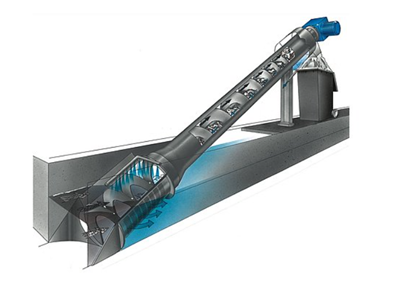
\includegraphics[width=1\textwidth]{Figurar/Grovrist.png.png}
    \caption{Illustrasjon Huber Grovrist}\label{fig:Huber Grovrist}
\end{figure}
    
